%% LyX 2.1.4 created this file.  For more info, see http://www.lyx.org/.
%% Do not edit unless you really know what you are doing.
\documentclass[british,aps,prl,superscriptaddress,nofootinbib,times,reprint]{revtex4-1}
\usepackage[T1]{fontenc}
\usepackage[latin9]{inputenc}
\usepackage{geometry}
\geometry{verbose,tmargin=2cm,bmargin=2cm,lmargin=2cm,rmargin=2cm,headheight=2cm,headsep=2cm,footskip=2cm}
\setcounter{secnumdepth}{3}
\usepackage{verbatim}
\usepackage{refstyle}
\usepackage{amsmath}
\usepackage{amsthm}
\usepackage{amssymb}
\usepackage{esint}

\makeatletter

%%%%%%%%%%%%%%%%%%%%%%%%%%%%%% LyX specific LaTeX commands.

\AtBeginDocument{\providecommand\thmref[1]{\ref{thm:#1}}}
\AtBeginDocument{\providecommand\lemref[1]{\ref{lem:#1}}}
\AtBeginDocument{\providecommand\propref[1]{\ref{prop:#1}}}
\AtBeginDocument{\providecommand\eqref[1]{\ref{eq:#1}}}
\AtBeginDocument{\providecommand\figref[1]{\ref{fig:#1}}}
\AtBeginDocument{\providecommand\secref[1]{\ref{sec:#1}}}
\AtBeginDocument{\providecommand\ssecref[1]{\ref{ssec:#1}}}


\newref{sec}{name=Section~}
\newref{ssec}{name=Subsection~}

\RS@ifundefined{subref}
  {\def\RSsubtxt{section~}\newref{sub}{name = \RSsubtxt}}
  {}
\RS@ifundefined{thmref}
  {\def\RSthmtxt{Theorem~}\newref{thm}{name = \RSthmtxt}}
  {}
\RS@ifundefined{lemref}
  {\def\RSlemtxt{Lemma~}\newref{lem}{name = \RSlemtxt}}
  {}
\RS@ifundefined{propref}
  {\def\RSproptxt{Proposition~}\newref{prop}{name = \RSproptxt}}
  {}


%%%%%%%%%%%%%%%%%%%%%%%%%%%%%% Textclass specific LaTeX commands.
\theoremstyle{plain}
\newtheorem{thm}{\protect\theoremname}
  \theoremstyle{definition}
  \newtheorem{defn}[thm]{\protect\definitionname}
  \theoremstyle{remark}
  \newtheorem{rem}[thm]{\protect\remarkname}
  \theoremstyle{plain}
  \newtheorem*{prop*}{\protect\propositionname}
  \theoremstyle{plain}
  \newtheorem{lem}[thm]{\protect\lemmaname}
  \theoremstyle{plain}
  \newtheorem{prop}[thm]{\protect\propositionname}
  \theoremstyle{definition}
  \newtheorem{example}[thm]{\protect\examplename}
  \theoremstyle{definition}
  \newtheorem{notn}[thm]{\protect\notationname}

%%%%%%%%%%%%%%%%%%%%%%%%%%%%%% User specified LaTeX commands.
\usepackage{graphicx}
\graphicspath{ {images/} }

\usepackage{xcolor}
%\usepackage{url}
\usepackage{hyperref}
\hypersetup{
    colorlinks,
    linkcolor={red!50!black},
    citecolor={blue!50!black},
    urlcolor={blue!80!black}
}

\makeatother

\usepackage{babel}
  \providecommand{\definitionname}{Definition}
  \providecommand{\examplename}{Example}
  \providecommand{\lemmaname}{Lemma}
  \providecommand{\propositionname}{Proposition}
  \providecommand{\remarkname}{Remark}
  \providecommand{\theoremname}{Theorem}
  \providecommand{\notationname}{Notation}

\begin{document}

\title{A non-contextual hidden variable model for Quantum Mechanics}


\author{Atul Singh Arora}

\email{ms11003@iisermohali.ac.in}

\selectlanguage{british}%

\affiliation{Indian Institute of Science Education and Research (IISER), Mohali}


\author{Arvind}

\email{arvind@iisermohali.ac.in}

\selectlanguage{british}%

\affiliation{Indian Institute of Science Education and Research (IISER), Mohali}
\begin{abstract}
We propose a non-contextual hidden variable model, consistent with all predictions of Quantum Mechanics (QM). We reconsider the no-go theorems on hidden variables and conclude that the notion of contextuality is not a necessary feature of QM. Motivated by consistency requirements between Bohmian Mechanics and the said theorems, we provide an alternative view. This is accomplished by identifying a new classical property, we call `multiplicativity'. It turns out that if this condition is relaxed one is able to construct hidden variable models which are consistent with QM. Advantages of this view are illustrated by considering the implications of non-multiplicativity to non-locality. Our model is for finite dimensional quantum systems, however, generalization to the infinite dimensional case should be possible. %and its relation to contextuality.
\end{abstract}
\maketitle

\section{Introduction}

Einstein's \cite{EinsteinEPR} work on incompleteness of QM and the subsequent seminal work of Bell \cite{Bell1964}, assessing compatibility of hidden variable (HV) models with QM has proven to be repeatedly useful. In Bell's case, for instance, it gave a precise meaning to the foundational notion of locality. Further, it has been of pragmatic utility in the areas of security, randomness certification etc. \cite{Ekert,PironioRndmnssCrtfcn} While Bell showed that local HV models can not describe nature, the Kochen Specker theorem \cite{KochenSpecker} (and related work \cite{Gleason,BellOnHiddenVariables,Peres,Mermin}) ruled out an even larger class of HV models. Consequently the notion of contextuality was identified, methods to experimentally test it were proposed and evidence in its favour reported \cite{SimonContExpProp,HuangContExp,YangContExp,HasegawaContExp}. Contextuality also, in recent times has been harnessed for computation and cryptography \cite{HowardCntxCmptn,CabelloCntxScrt}. []Contextuality has also stirred further investigation of foundational aspects of QM: relation between contextuality and classicality has been explored \cite{PawelCntxClsscl}, contextuality has been quantified in terms of memory \cite{MatthiasCntxMmry} and bounded memory in conjunction with contextuality has been used to show completeness of QM \cite{CabelloMmryQM}.[] Not all HV models were, however, proved to be incompatible by the aforesaid theorem. Bohm's work \cite{Bohm1,Bohm2} is one such (in)famous example. This approach has allowed for an interpretation of QM with precise trajectories.


%Previous work {[}the essentials I have already discussed{]}: 
We take a closer look at the aforesaid no-go theorems and find that contextuality is in fact not a necessary feature of QM (see \figref{block}). This has been shown earlier by taking disturbances due to measurements into consideration \cite{NoContextuality,LaCourNoCntx}. In this paper, we construct a significantly simpler toy model for illustrating not only the aforesaid but to also delineate a complete alternative to contextuality. The toy model is a specific case of what we call a c-ingle variable theory. Its predictions match with those of QM for systems described by arbitrary finite dimensional Hilbert spaces.

%Triangle: <TODO: ask arvind sir, see \figref{block}>

\begin{figure}[h]
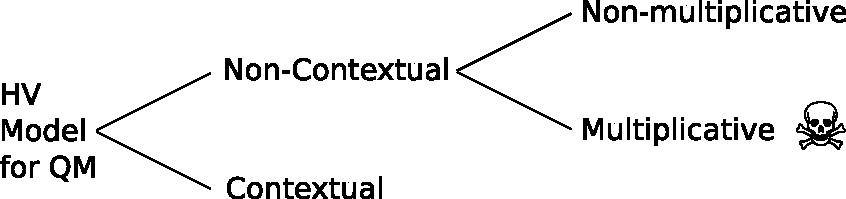
\includegraphics[width=\columnwidth]{block1}
\caption{Non-contextuality is not inconsistent with QM}
\label{fig:block}\end{figure}

Organization of this paper is as follows. In \secref{context} we establish a notation and definitions to facilitate further discussions. In \secref{nonMultiplicativity} we introduce the notion of multiplicativity and that of sequential multiplicativity. We review the `contextuality' theorem and prove some results about multiplicativity. We construct an explicit non-contextual model in \ssecref{cingle} and apply it to the very proof of `contextuality' to illustrate non-multiplicativity. This is supplemented by a discussion about Bohmian Mechanics in \ssecref{nonContBohm} where contextuality is removed by hand. The paper is concluded with discussion of implications of multiplicativity on locality, entanglement, superposition and apparent contextuality in \secref{implications}.


\section{Context \label{sec:context}}

The notation used henceforth has been defined below.


\begin{notn} (a) $\psi\in\mathcal{H}$ would typically represent the quantum mechanical state of the system (assumed pure), residing in the Hilbert space $\mathcal{H}$, (b) $\hat{\mathcal{H}}$ is defined to mean $\mathcal{H}\otimes\mathcal{H}^{\dagger}$ (i.e. the set of Hermitian operators, observables, on the space $\mathcal{H}$), (c) $[\mathcal{H}]$ is defined to mean $(\mathcal{H},\,\mathbb{R}^{\otimes})$, which represents the state of the system including HVs, (d) $[\psi]\in[\mathcal{H}]$ will represent the state of the system, including HVs, (e) a prediction map is $m:\hat{\mathcal{H}},[\mathcal{H}]\to\mathbb{R}$, (f) a sequence map is $s:\hat{\mathcal{H}},[\mathcal{H}],\mathbb{R}\to[\mathcal{H}]$, (g) $f$ is an arbitrary map from $\{ \hat{\mathcal{H}},\hat{\mathcal{H}},\dots\hat{\mathcal{H}} \} \to \hat{\mathcal{H}}$ constructed using multiplication and addition of the observables, and multiplication with complex numbers\footnote{Strictly, the map $f$ would depend on the operators to ensure preservation of Hermiticity; thus a given $f$ will be defined only for a subset of $\{ \hat{\mathcal{H}},\hat{\mathcal{H}},\dots\hat{\mathcal{H}} \}$.}, (h) $\tilde{f}$ is a map constructed by replacing observables in $f$ with real numbers. 
%\footnote{$\tilde f$ constructed this way should be written as $\tilde f:\mathbb{R}^{\otimes N} \to \mathbb{C}$. In fact the values should be restricted to the spectrum of the associated observables.}.
\end{notn}

In addition to the notation, we use the following definition of non-contextuality.
\begin{defn}
A theory is non-contextual, if it provides a map $m: \{ \hat{\mathcal{H}},[\mathcal{H}] \} \to\mathbb{R}$ to explain measurement outcomes. A theory which is not non-contextual is contextual.\end{defn}
\begin{rem}
The notion of non-contextuality may be extended to maps. A map is non-contextual if it is of the form $m: \{ \hat{\mathcal{H}},[\mathcal{H}] \} \to\mathbb{R}$; prediction maps are non-contextual.
\end{rem}

In the literature broader definitions have been suggested which declare a larger set of theories as non-contextual. For our purposes however, this restricted definition will suffice. The term contextual is used to suggest that the value an operator takes might depend on which other compatible observable it is measured with.


\section{Non-Multiplicativity: An alternative to Contextuality \label{sec:nonMultiplicativity}}

One can show \cite{KochenSpecker} that under reasonable assumptions, no non-contextual theory can explain all predictions of QM. We re-state these results and show that nowhere does contextuality appear to be a logical necessity. Instead we note that non-contextual theories with certain properties, we call \emph{multiplicativity} are incompatible with QM. Viewed from this perspective, non-\emph{multiplicativity} is the non-classical alternative to contextuality in QM. Precise definitions of this and a related property \emph{sequential multiplicativity}, are given below. 

\begin{defn}
A prediction map $m$ is \emph{multiplicative} iff 
% \[
% \begin{split}
% m(f(\hat{B}_{1},\hat{B}_{2},\dots\hat{B}_{N}),[\psi]) = \\
% f(m(\hat{B}_{1},[\psi]),m(\hat{B}_{2},[\psi]),\dots m(\hat{B}_{N},[\psi])),
% \end{split}
% \]

\begin{align*}
& m(f(\hat{B}_{1},\hat{B}_{2},\dots\hat{B}_{N}),[\psi]) = \\
& \tilde f(m(\hat{B}_{1},[\psi]),m(\hat{B}_{2},[\psi]),\dots m(\hat{B}_{N},[\psi])),
\end{align*}
where $\hat{B}_{i}\in\hat{\mathcal{H}}$ are arbitrary mutually commuting observables and $[\psi]\in[\mathcal{H}]$. A non-\emph{multiplicative} map is one that is not multiplicative.
\end{defn}
Note that if $m$ is taken to represent the measurement outcome (in
QM), then for states of the system which are simultaneous eigenkets
of $\hat{B}_{i}$s, $m$ must clearly be multiplicative. It is, however,
not obvious that this property must always hold. To motivate this,
consider the state of two spin half particles, $\left|11\right\rangle :=\left|1\right\rangle \otimes\left|1\right\rangle $
written in the computational basis, $\hat{B}_{1}=\hat{\sigma}_{x}\otimes\hat{\sigma}_{x}$,
$\hat{B}_{2}=\hat{\sigma}_{y}\otimes\hat{\sigma}_{y}$ and $\hat{C}=\hat{B}_{1}\hat{B}_{2}=-\hat{\sigma}_{z}\otimes\hat{\sigma}_{z}$.
We must have $m(\hat{C})=-1$ while $m(\hat{B}_{1})=\pm1$ and $m(\hat{B}_{2})=\pm1$,
independently, according to QM, with probability half. Here multiplicativity doesn't seem to hold. Antithetically it is clear that if one first measures
$\hat{B}_{1}$ and subsequently measures $\hat{B}_{2}$, then the
product of the results must be $-1$. This is consistent with measuring
$\hat{C}$. To capture this property we define \emph{sequential multiplicativity}
as follows.
\begin{defn}
A prediction map $m$ is \emph{sequentially multiplicative} for a
given sequence map $s$, iff 
\begin{align*}
&m(f(\hat{B}_{1},\hat{B}_{2},\dots\hat{B}_{N}),[\psi_{1}])=\\
&\tilde f(m(\hat{B}_{1},[\psi_{k_{1}}]),m(\hat{B}_{2},[\psi_{k_{2}}]),\dots,m(\hat{B}_{N},[\psi_{k_{N}}])),
\end{align*}
where $\mathbf{k}=(k_{1},k_{2},\dots,k_{N})\in\{(1,2,3\dots N),(2,1,3\dots N)$ + permutations, making $N!$ terms$\}$,
$\hat{B}_{i}\in\hat{\mathcal{H}}$ are arbitrary mutually commuting
observables, $[\psi_{i}]\in[\mathcal{H}]$ and $[\psi_{k+1}]\equiv s(\hat{B}_{k},[\psi_{k}],m(\hat{B}_{k},[\psi_{k}]))$,
$\forall\,[\psi_{i}]$.
\end{defn}
We now discuss the `proofs of contextuality' in the purview of the
aforesaid.
\begin{thm}
Let a map $m:\hat{\mathcal{H}}\to\mathbb{R}$, be s.t. (a) $m(\hat{\mathbb{I}})=1$,
(b) $m(f(\hat{A}_{1},\hat{A}_{2},\dots))=\tilde f(m(\hat{A}_{1}),m(\hat{A}_{2}),\dots)$,
where $\hat{A}_{i}$ are arbitrary Hermitian operators. If $m$ is assumed to describe the outcomes of measurements, then no $m$ exists which is consistent with all predictions of QM\label{thm:det} (see \ref{proofs} for proofs). \end{thm}
Here $m$ maybe viewed as a specific class of prediction maps, that
implicitly depends on the state $[\psi]$. It follows then that the
maps ruled out by the theorem are non-contextual. The set of maps
ruled out, however, can be enlarged by imposing fewer restrictions
on it. This is achieved by the following theorem.

\begin{thm}
Let a map $m:\hat{\mathcal{H}}\to\mathbb{R}$, be s.t. (a) $m(\hat{\mathbb{I}})=1$,
(b) $m(f(\hat{B}_{1},\hat{B}_{2},\dots))=\tilde f(m(\hat{B}_{1}),m(\hat{B}_{2}),\dots)$,
for any arbitrary function $f$, where $\hat{B}_{i}$ are mutually
commuting Hermitian operators. If $m$ is assumed to describe the
outcomes of measurements, then no $m$ exists which is consistent
with all predictions of QM (see \ref{proofs} for more proofs).\label{thm:KS}\end{thm}


% The following proof is not only more general, but also independent
% of the initial state of the system.
\begin{proof}
Peres Mermin ($\left|\mathcal{H}\right|\ge4$) \cite{Peres,Mermin}:

Consider the following set of operators 
\[
\hat{A}_{ij}\doteq\left[\begin{array}{ccc}
\hat{\mathbb{I}}\otimes\hat{\sigma}_{x} & \hat{\sigma}_{x}\otimes\hat{\mathbb{I}} & \hat{\sigma}_{x}\otimes\hat{\sigma}_{x}\\
\hat{\sigma}_{y}\otimes\hat{\mathbb{I}} & \hat{\mathbb{I}}\otimes\hat{\sigma}_{y} & \hat{\sigma}_{y}\otimes\hat{\sigma}_{y}\\
\hat{\sigma}_{y}\otimes\hat{\sigma}_{x} & \hat{\sigma}_{x}\otimes\hat{\sigma}_{y} & \hat{\sigma}_{z}\otimes\hat{\sigma}_{z}
\end{array}\right]
\]
which have the property that all operators along a row (or column) commute and that the product of rows (or columns) yield $\hat{R}_{i}=\mathbb{I}$ and $\hat{C}_{j}=\mathbb{I}\,(j\neq3)$, $\hat{C}_{3}=-\mathbb{I}$, ($\forall\,i,j$) where $\hat{R}_{i}\equiv\prod_{j}\hat{A}_{ij}$, $\hat{C}_{j}\equiv\prod_{i}\hat{A}_{ij}$. Let us assume that $m$ exists. From property (b) of the map, to get $m(\hat{C}_{3})=-1$ (as required by property (a)), we must have an odd number of $-1$ assignments in the third column. In the remaining columns, the number of $-1$ assignments must be even (for each column). Thus, in the entire square, the number of $-1$ assignments must be odd. Let us use the same reasoning, but along the rows. Since each $m(\hat{R}_{i})=1$, we must have even number of $-1$ assignments along each row. Thus, in the entire square, the number of $-1$ assignments must be even. We have arrived at a contradiction and therefore we conclude that our assumption that a consistent $m$ exists, must be wrong.
\end{proof}

\begin{rem}
One could in principle assume $m$, to be s.t. (a) $m(\hat{\mathbb{I}})=1$,
(b) $m(\alpha\hat{B}_{i})=\alpha m(\hat{B}_{i})$, for $\alpha\in\mathbb{R}$,
(c) $m(\hat{B}_{i}^{2})=m(\hat{B}_{i})^{2}$, (d) $m(\hat{B}_{i}+\hat{B}_{j})=m(\hat{B}_{i})+m(\hat{B}_{j})$,
to deduce (d') $m(\hat{B}_{i}\hat{B}_{j})=m(\hat{B}_{i})m(\hat{B}_{j})$
and that $m(\hat{B}_{i})\in$ spectrum of $\hat{B}_{i}$. Effectively
then, condition (b) listed in the theorem is satisfied as a consequence.
Therefore, assuming (a)-(d) as listed here, rules out a larger class
of $m$. \cite{KochenSpecker}
\end{rem}
According to \thmref{KS}, non-contextual maps which are \emph{multiplicative}
must be incompatible with QM. It is apparent that non-contextual maps
which are non-\emph{multiplicative} might be consistent with QM. To
that end, in the following section we first show that this is indeed
the case by constructing an explicit model and supplement it by removing contextuality from Bohmian Mechanics.

Before proceeding we note, however, that QM can enforce \emph{sequential multiplicativity}. This result will be used to assess accuracy of any HV model we might propose.
\begin{prop*}
Let the system be in a state, s.t. measurement of $\hat{C}$ yields
repeatable results (same result each time). Then according to QM,
\emph{sequential multiplicativity} holds, where $\hat{C}\equiv f(\hat{B}_{1},\hat{B}_{2},\dots\hat{B}_{n})$,
and $\hat{B}_{i}$ are as defined. \end{prop*}
\begin{proof}
Assume without loss of generality that $\hat{B}_{1},\hat{B}_{2},\dots\hat{B}_{n}$
are mutually compatible (commuting) and complete set of operators.
If say for instance the set is not complete, then one can add the
missing operators and label them as aforesaid. It follows that $\exists$
$\left|\mathbf{b}=\left(b_{1}^{(l_{1})},b_{2}^{(l_{2})},\dots b_{n}^{(l_{n})}\right)\right\rangle $
s.t. $\hat{B}_{i}\left|\mathbf{b}\right\rangle =b_{i}^{(l_{i})}\left|\mathbf{b}\right\rangle $,
where $l_{i}$ indexes the eigenvalues corresponding to $\hat{B}_{i}$
and that $\sum_{\mathbf{b}}\left|\mathbf{b}\right\rangle \left\langle \mathbf{b}\right|=\hat{\mathbb{I}}$.
Let the state of the system be given by $\left|\psi\right\rangle $
and it must be s.t. $\hat{C}\left|\psi\right\rangle =c\left|\psi\right\rangle $,
by assumption. For the statement to follow, one need only show that
$\left|\psi\right\rangle $ must be made of only those $\left|\mathbf{b}\right\rangle $s,
which satisfy $c=\tilde f(b_{1}^{(l_{1})},b_{2}^{(l_{2})},\dots b_{n}^{(l_{n})})$.
This is the crucial step. Proving this is so is trivial. We start
with $\hat{C}\left|\psi\right\rangle =c\left|\psi\right\rangle $
and take its inner product with $\left\langle \mathbf{b}\right|$
to get 
\begin{eqnarray*}
\left\langle \mathbf{b}\right|\hat{C}\left|\psi\right\rangle  & = & c\left\langle \mathbf{b}|\psi\right\rangle ,\\
\left\langle \mathbf{b}\right|f(\hat{B}_{1},\hat{B}_{2},\dots\hat{B}_{n})\left|\psi\right\rangle  & = & c\left\langle \mathbf{b}|\psi\right\rangle ,\\
\tilde f(b_{1}^{(l_{1})},b_{2}^{(l_{2})},\dots b_{n}^{(l_{n})})\left\langle \mathbf{b}|\psi\right\rangle  & = & c\left\langle \mathbf{b}|\psi\right\rangle .
\end{eqnarray*}
Also, we have $\left|\psi\right\rangle =\sum_{\mathbf{b}}\left\langle \mathbf{b}|\psi\right\rangle \left|\mathbf{b}\right\rangle $, from completeness. If we consider $\left|\mathbf{b}\right\rangle $s for which $\left\langle \mathbf{b}|\psi\right\rangle \neq0$, then we can conclude that indeed $c=\tilde f(b_{1}^{(l_{1})},b_{2}^{(l_{2})},\dots b_{n}^{(l_{n})})$. However, when $\left\langle \mathbf{b}|\psi\right\rangle =0$, viz. $\left|\mathbf{b}\right\rangle $s that are orthogonal to $\left|\psi\right\rangle $, then nothing can be said. We can thus conclude that $\left|\psi\right\rangle $ is made only of those $\left|\mathbf{b}\right\rangle $s that satisfy the required relation. That completes the proof.
\end{proof}
It is worth noting that in the PM case, where $\hat{R}_{i}$ and $\hat{C}_{j}$ are just $\pm\hat{\mathbb{I}}$, it follows that all states are their eigenstates. Consequently, for these operators \emph{sequential multiplicativity} must always hold.

\subsection{C-ingle model | An Explicit Construction \label{ssec:cingle}}

Let the state of the system be $\left|\chi\right\rangle $, defined on a finite dimensional Hilbert space and we wish to assign a value to an arbitrary observable $\hat{A}=\sum_{a}a\left|a\right\rangle \left\langle a\right|$, which has eigenvalues $\{a_{\text{min}}=a_{1}\le a_{2}\dots\le a_{n}=a_{\text{max}}\}$. This model has the following postulates: \\
1. Initial HV: Pick a $c\in[0,1]$, from a uniform random distribution.\\
2. Assignment/Prediction: The value assigned to $\hat{A}$ is given by finding the smallest $a$ s.t. 
\[
c\le\sum_{a'=a_{\text{min}}}^{a}\left|\left\langle a'|\chi\right\rangle \right|^{2},
\]
viz. we have specified a prediction map, $m(\hat{A})=a$.\\
3. Update: After measuring an operator, the state is updated (collapsed) in accordance with the rules of QM. This completely specifies the sequence map $s$.

To see how this works, we restrict ourselves to a single spin half particle. Say $\left|\chi\right\rangle =\cos\theta\left|0\right\rangle +\sin\theta\left|1\right\rangle $, and $\hat{A}=\hat{\sigma}_{z}=\left|0\right\rangle \left\langle 0\right|-\left|1\right\rangle \left\langle 1\right|$. Now, according to the postulates of this theory, $m(\hat{A})=+1$, if $c\le\cos^{2}\theta$ else $\hat{A}$ is assigned $-1$. It follows then, from $c$ being uniformly random in $[0,1]$ that the statistics agree with predictions of QM. The reader can convince him(her)self that the said scheme works in general. 

Note that the assignment, described by the prediction map $m$, is non-contextual since given an operator and a state (+ the HV), the value is uniquely assigned. The map $m$ is, however, non-multiplicative which is clarified by the following non-trivial example.
\begin{example}
C-ingle model applied to the Peres Mermin situation: For illustration, let us start with the state $\left|\psi_{1}\right\rangle =\left|00\right\rangle $. Say from a uniform random distribution we obtained $c=0.4$. To arrive at the assignments, note that $\left|00\right\rangle $ is an eigenket of only $\hat{R}_{i},\hat{C}_{j}$ and $\hat{A}_{33}=\hat{\sigma}_{z}\otimes\hat{\sigma}_{z}$.
Thus, in the first iteration, all these should be assigned their respective eigenvalues. The remaining operators must be assigned $-1$ as one can readily verify by explicitly finding the smallest $a$ as described in postulate 2 of the model (see \eqref{toyModel}). Two remarks are in order. First, this model is manifestly \emph{non-multiplicative}, for $m_{1}(\hat{C}_{3})=1\neq m_{1}(\hat{A}_{13})m_{1}(\hat{A}_{23})m_{1}(\hat{A}_{33})=-1$, where the subscript has been introduced to index the iteration. More precisely, $m_{1}(\hat{O}):=m(\hat{O},\left[\left|\psi_{1}\right\rangle =\left|00\right\rangle \right])$ where the complete state $\left[\left|\psi_{1}\right\rangle \right]$ implicitly refers to both the quantum state $\left|00\right\rangle $ and the HV $c=0.4$. Second, we must impose \emph{sequential multiplicativity} as a consistency check of the model, which in particular entails that $m_{1}(\hat{C}_{3})=m_{1}(\hat{A}_{33})m_{2}(\hat{A}_{23})m_{3}(\hat{A}_{13})$, where $m_{2}:=m(\hat{O},\left[\left|\psi_{2}\right\rangle \right])$, $m_{3}:=m(\hat{O},\left[\left|\psi_{3}\right\rangle \right])$ and
$\left|\psi_{2}\right\rangle ,\,\left|\psi_{3}\right\rangle $ are obtained from postulate 3. Note that for each iteration, a new HV is generated. To illustrate \emph{sequential multiplicativity}, we must choose to measure $\hat{A}_{33}$. According to step 3, since $\left|00\right\rangle $ is an eigenstate of $\hat{A}_{33}$, the final state remains $\left|00\right\rangle $. 
\end{example}
\begin{widetext}
\begin{equation}
\begin{array}{c|ccc}
\text{Iteration} & i=1 & i=2 & i=3\\
\left|\psi_{\text{init}}\right\rangle  & \left|00\right\rangle  & \left|00\right\rangle  & \frac{\left|00\right\rangle +\left|11\right\rangle }{\sqrt{2}}\\
\text{HV/Toss} & c=0.4 & c=0.1 & c=0.7\\
\\
\text{Predictions} & m_{1}(\hat{A}_{ij})\doteq\left[\begin{array}{ccc}
-1 & -1 & -1\\
-1 & -1 & -1\\
-1 & -1 & +1
\end{array}\right] & m_{2}(\hat{A}_{ij})\doteq\left[\begin{array}{ccc}
-1 & -1 & -1\\
-1 & -1 & -1\\
-1 & -1 & +1
\end{array}\right] & m_{3}(\hat{A}_{ij})\doteq\left[\begin{array}{ccc}
+1 & +1 & +1\\
+1 & +1 & -1\\
+1 & +1 & +1
\end{array}\right]\\
\text{(Assignments)}\\
 & m_{1}(\hat{R}_{i}),m_{1}(\hat{C}_{j})=+1\,(j\neq3) & m_{2}(\hat{R}_{i}),m_{2}(\hat{C}_{j})=+1\,(j\neq3) & m_{3}(\hat{R}_{i}),m_{3}(\hat{C}_{j})=+1\,(j\neq3)\\
 & m_{1}(\hat{C}_{3})=-1 & m_{2}(\hat{C}_{3})=-1 & m_{3}(\hat{C}_{3})=-1\\
\text{Operator}\\
\text{Measured} & \hat{A}_{13}=\hat{\sigma}_{z}\otimes\hat{\sigma}_{z};m_{1}(\hat{A}_{13})=+1 & \quad\quad\hat{A}_{23}=\hat{\sigma}_{y}\otimes\hat{\sigma}_{y};m_{2}(\hat{A}_{23})=-1\quad\quad & \hat{A}_{33}=\hat{\sigma}_{x}\otimes\hat{\sigma}_{x};m_{3}(\hat{A}_{33})=+1\\
\\
\left|\psi_{\text{final}}\right\rangle  & \left|00\right\rangle  & \frac{\left|00\right\rangle +\left|11\right\rangle }{\sqrt{2}} & \frac{\left|00\right\rangle +\left|11\right\rangle }{\sqrt{2}}
\end{array}\label{eq:toyModel}
\end{equation}
\end{widetext}
For the next iteration, $i=2$, viz. after the first measurement has
been performed, say the random number generator yielded $c=0.1$.
Since $\left|\psi\right\rangle $ is also unchanged the assignment
remains invariant (in fact any of $c<0.5$ would yield the same result),
which should be evident from the previous exercise. For the final
step we choose to measure $\hat{p}:=\hat{A}_{23}(=\hat{\sigma}_{y}\otimes\hat{\sigma}_{y})$,
to proceed with sequentially measuring $\hat{C}_{3}$. To simplify
calculations, we note 
\[
\left|00\right\rangle =\frac{(\left|\tilde{+}\tilde{-}\right\rangle +\left|\tilde{-}\tilde{+}\right\rangle )/\sqrt{2}+(\left|\tilde{+}\tilde{+}\right\rangle +\left|\tilde{-}\tilde{-}\right\rangle )/\sqrt{2}}{\sqrt{2}},
\]
where $\left|\tilde{\pm}\right\rangle =\left|0\right\rangle \pm i\left|1\right\rangle $
(eigenkets of $\hat{\sigma}_{y}$). Since $\left|00\right\rangle $
is manifestly not an eigenket of $\hat{p}$, we must find an appropriate
eigenket $\left|p_{-}\right\rangle $ s.t. $\hat{p}\left|p_{-}\right\rangle =-\left|p_{-}\right\rangle $,
since $c=0.1$ and $\left\langle p_{-}|00\right\rangle $ is already
$>0.1$. It is immediate that $\left|p_{-}\right\rangle =\left(\left|\tilde{+}\tilde{-}\right\rangle +\left|\tilde{-}\tilde{+}\right\rangle \right)/\sqrt{2}=\left(\left|00\right\rangle +\left|11\right\rangle \right)/\sqrt{2}$,
which becomes the final state. \\
For the final iteration, $i=3$, say we obtain $c=0.7$. So far, we
have $m_{1}(\hat{A}_{33})=1$ and $m_{2}(\hat{A}_{23})=-1$. We must
obtain $m_{3}(\hat{A}_{13})=1$, independent of the value of $c$,
to be consistent. Let's check that. Indeed, according to postulate
2, since $\hat{\sigma}_{x}\otimes\hat{\sigma}_{x}\left(\left|00\right\rangle +\left|11\right\rangle \right)/\sqrt{2}=1\left(\left|00\right\rangle +\left|11\right\rangle \right)/\sqrt{2}$,
$m_{3}(\hat{A}_{13})=1$ for all allowed values of $c$. As a remark,
it maybe emphasised that the $m_{2}(\hat{A}_{33})=m_{3}(\hat{A}_{33})$
and $m_{2}(\hat{A}_{23})=m_{3}(\hat{A}_{23})$, which essentially
expresses compatibility of these observables, viz. measurement of
$\hat{A}_{13}$ doesn't affect the result one would obtain by measuring
operators compatible to it (granted they have been measured once before).


\subsection{Non-contextual Bohmain Mechanics \label{ssec:nonContBohm}}

Since QM yields deterministic results only in specific situations, it is imperative to analyse the meaning of contextuality by `completing' QM. HV theories do precisely this and we have at our disposal the heretic theory of Bohm. Circumventing the details of the theory, we note its salient feature; with each particle, one associates precisely defined $(q,p)$ and a wavefunction $\psi$. The construction is such that the particles are guided by the wavefunction. Consequently, the outcomes of all experiment are predictable, granted the initial conditions of the system and the apparatus are known (the `HV'). The essence of Bohmian Mechanics relevant here can be captured by the following theorem.

\begin{defn}
(a) the set of all experimental setups is denoted by $\mathcal{E}$, (b) a setup map is $e:\hat{\mathcal{H}}\to\mathcal{E}$.
\end{defn}

\begin{thm}
$\exists$ a (Bohmian) map $m_{B}:\hat{\mathcal{H}},[\mathcal{H}],\mathcal{E}\to\mathbb{R}$, and a sequence map $s$, s.t. if $m_{B}$ \& $s$ are assumed to describe the outcomes of measurements \& the resultant state respectively, then they are consistent with all predictions of QM.
\end{thm}
Observe that given a Stern-Gerlach setup and the initial conditions (position \& wavefunction of the particle), according to the theorem, Bohmian mechanics can predict the value of the spin (say $\hat{\sigma}_{z}$) of the particle. Assume that the state of the particle was $(\left|0\right\rangle +\left|1\right\rangle )/\sqrt{2}$ and that the measurement outcome was spin up. Interestingly, it has be shown that if the direction of the magnetic field gradient is flipped while everything else is unchanged, the measurement outcome will now be spin down \cite{Detlef}. This emphasises the fact that $m_{B}$ is not a prediction map. More importantly it entails that $m_{B}$ is contextual. It must be stressed, however, that the contextuality in this case is not a statement about the context in terms of compatible observables. Here no two observables are compatible (excluding identity).
Contextuality in Bohmian Mechanics arises from the mapping between an operator and the experimental setup. Consider, however, the following proposition.
\begin{lem}
For finite dimensional $\mathcal{H}$, $\exists$ a map $e:\hat{\mathcal{H}}\to\mathcal{E}$. \label{lem:OpeExp} (See \ref{proofs})
\end{lem}
The proof of this proposition can be motivated by a simple construction. Consider that the system of interest are spin half particles. To measure spin along any direction, there are two directions along which the magnetic field gradient can be set (as was discussed in the introduction). The experimentalist agrees to always use a specific direction, thereby mapping an operator to an experimental setup uniquely. Given this, one can immediately derive a consistent non-multiplicative prediction map $m$.
\begin{prop}
The Bohmian map, $m_{B}$ can be restricted to a prediction map $m$, we call `Bohmian prediction map'.
\end{prop}
\begin{proof}
$m(\hat{\mathcal{H}},[\mathcal{H}])=m_{B}(\hat{\mathcal{H}},[\mathcal{H}],e(\hat{\mathcal{H}}))$.
\end{proof}
\begin{prop}
The Bohmian prediction map, $m$ must be non-multiplicative.
\end{prop}
\begin{proof}
Since Bohmian Mechanics is consistent with all predictions of QM, the Bohmian prediction map $m$ must also be. According to \thmref{KS}, $m$ must be non-multiplicative.
\end{proof}

\section{Concluding Remarks \label{sec:implications}}


\subsection{Locality}


\begin{defn}
A theory/model/map is \emph{local} iff two spatially distinct points can not be influenced instantaneously.
\end{defn}

\begin{prop}
A prediction map $m$ consistent with QM must be non-local \label{prop:predMapNonLocal} (see \ref{proofs} for details).
\end{prop}

\begin{prop}
Consider a product Hilbert space $\mathcal{H}_{A}\otimes\mathcal{H}_{B}$, corresponding to two particles. $\mathcal{H}_{A}$ and $\mathcal{H}_{B}$ are finite dimensional. Let mutually commuting observables $\hat{B}_{i}$ be s.t. $\hat{B}_{i}=\hat{\mathbb{I}}\otimes\hat{A}_{\text{B}i}$ or $\hat{B}_{i}=\hat{A}_{\text{A}i}\otimes\hat{\mathbb{I}}$, where $A_{\text{A}i}\in\mathcal{\hat{H}}_{A}$ and $A_{\text{B}i}\in\hat{\mathcal{H}}_{B}$ are arbitrary observables. If locality is assumed, then a prediction map $m$ and it's associated sequence map $s$ must be s.t. over these observables, sequential multiplicativity and multiplicativity become identical.
\end{prop}



\subsection{Apparent Contextuality}

We have already constructed an explicit non-contextual model, which
is consistent with QM. This model we knew had to be non-multiplicative.
We will see how non-multiplicativity gives rise to what one might
confuse to mean contextuality. Imagine 
\[
\hat{B}_{1}=\hat{\sigma}_{z}\otimes\hat{\mathbb{I}}=\left|00\right\rangle \left\langle 00\right|+\left|01\right\rangle \left\langle 01\right|-\left[\left|10\right\rangle \left\langle 10\right|+\left|11\right\rangle \left\langle 11\right|\right],
\]
\[
\hat{B}_{2}=\hat{\mathbb{I}}\otimes\hat{\sigma}_{z}=\left|10\right\rangle \left\langle 10\right|+\left|11\right\rangle \left\langle 11\right|-\left[\left|00\right\rangle \left\langle 00\right|+\left|01\right\rangle \left\langle 01\right|\right],
\]
while we define 
\begin{align*}
\hat{C}&=f(\{\hat{B}_{i}\}) \\ 
       &=0.\left|00\right\rangle \left\langle 00\right|+1.\left|01\right\rangle \left\langle 01\right|+2.\left|10\right\rangle \left\langle 10\right|+3.\left|11\right\rangle \left\langle 11\right|.
\end{align*}
$\hat{C}$ maybe viewed as a function of $\hat{B}_{1}$, $\hat{B}_{2}$
and other operators $\hat{B}_{i}$ which are constructed to obtain
a maximally commuting set. A measurement of $\hat{C}$, will collapse
the state into one of the states which are simultaneous eignkets of
$B_{1}$ and $B_{2}$. Consequently, from the observed value of $\hat{C}$,
one can deduce the values of $\hat{B}_{1}$ and $\hat{B}_{2}$. Now
consider $\sqrt{2}\left|\chi\right\rangle =\left|10\right\rangle +\left|01\right\rangle $,
for which $m_{1}(\hat{B}_{1})=1$, and $m_{1}(\hat{B}_{2})=1$, using
the C-ingle model, with $c<0.5$. However, $m_{1}(\hat{C})=1$, from
which one can deduce that $B_{1}$ was $+1$, while $B_{2}$ was $-1$.
This property itself, one may be tempted call contextuality, viz.
the value of $B_{1}$ depends on whether it is measured alone or with
the remaining $\{B_{i}\}$. However, it must be noted that $B_{1}$
has a well defined value, and so does $\hat{C}$. Thus by our accepted
definition, there's no contextuality. It is just that $m_{1}(\hat{C})\neq f(m_{1}(\hat{B}_{1}),m_{1}(\hat{B}_{2}),\dots)$,
viz. the theory is non-multiplicative. Note that after measuring $\hat{C}$
however, $m_{2}(\hat{B}_{1})=+1$ and $m_{2}(\hat{B}_{2})=-1$ (for
any value of $c$) consistent with those deduced by measuring $\hat{C}$.


\subsection{Entanglement and Superposition}

It is known that for simultaneous eigenstates of $\hat{B}_{i}$, multiplicativity
must hold. Consequently, any violation of multiplicativity must arise
from states that are superpositions (of the simultaneous eigenkets).
Note however, that entanglement is not necessary to show a violation,
since, for example, the PM test is a state independent test, where
a separable state can be used to arrive at a contradiction. For demonstrating
non-locality using Bell's proof, however, it can be shown that entanglement
is necessary.

TODO: Discuss and complete.
\begin{appendix}
\section{Selected Proofs \label{proofs}}
Proofs of \thmref{det}:
\begin{proof}
Trivial yet most general proof ($\left|\mathcal{H}\right|\ge2$): Consider $\hat A _1 = \sigma_y$, $\hat A_2 =\sigma_x$, $\hat C = f(\hat A_1,\hat A_2) = i\hat A_1 \hat A_2=\sigma_z$. Now we know that $m(\hat \sigma_j)=\pm1$ which entails that $m(\hat C)=  im(\hat A_1)m(\hat A_2)=i$ where we have used property (b). However, $m(\hat C)=m(\hat \sigma_z)=\pm1$ which is a contradiction. Thus no consistent $m$ can exist.
\end{proof}

\begin{proof}
Bell construction ($\left|\mathcal{H}\right|\ge4$) \cite{Bell1964}: Consider an operator $\hat{B}:=a_{1}\otimes b_{1}+a_{2}\otimes b_{1}+a_{1}\otimes b_{2}-a_{2}\otimes b_{2}$ s.t. $-1\le\hat{a}_{i},\hat{b}_{j}\le1$ $\forall\,i,j\in\{1,2,3,4\}$ (which means that the spectrum of $\hat{a}$ and $\hat{b}$ are bounded above and below). If we assume that a map $m$ of the aforesaid type exists, then it can be shown that $\left\langle \hat{B}\right\rangle \le2$. To see this, consider $\hat{A}_{1}=\hat{a}_{1}\otimes\hat{\mathbb{I}}$ and $\hat{A}_{2}=\hat{\mathbb{I}}\otimes\hat{b}_{1}$, so that if $\hat{C}:=\hat{A}_{1}\hat{A}_{2}$ then property (2) entails that $m(\hat{C})=m(\hat{A}_{1})m(\hat{A}_{2})$, viz. $m(\hat{a}_{1}\otimes\hat{b}_{1})=m(\hat{a}_{1}\otimes\hat{\mathbb{I}})m(\hat{\mathbb{I}}\otimes\hat{b}_{1})$. Note that $m(\hat{*})$, may depend on the state $\left|\psi\right\rangle $ and the HVs. Therefore, we average over multiple measurements, which corresponds
to averaging over the HVs. This is expressed by $\left\langle m(\hat{a}_{1}\otimes\hat{b}_{1})\right\rangle =\left\langle m(\hat{a}_{1}\otimes\hat{\mathbb{I}})\right\rangle \left\langle m(\hat{\mathbb{I}}\otimes\hat{b}_{1})\right\rangle $. One can repeat this argument for each term in $\left\langle \hat{B}\right\rangle $. Using the fact that $-1\le m(\hat{*})\le1$, and that the extrema will occur only at the extreme values of $m$, one can plugin $\pm1$ for each $\left\langle m(\hat{*})\right\rangle $ to obtain $\left\langle \hat{B}\right\rangle \le2$. Quantum mechanically, one can show that $\left\langle \hat{B}\right\rangle =2\sqrt{2}$ for the state $\left|\psi\right\rangle =\left(\left|+-\right\rangle -\left|-+\right\rangle \right)/\sqrt{2}$,
where $\hat{\sigma}_{x}\left|\pm\right\rangle =\pm\left|\pm\right\rangle $, and $\hat{\sigma}_{x,y,z}$ are the Pauli matrices, given in the z-basis as  \[
\hat{\sigma}_{x}\doteq\left[\begin{array}{cc}
0 & 1\\
1 & 0
\end{array}\right],\,\hat{\sigma}_{y}\doteq\left[\begin{array}{cc}
0 & -i\\
i & 0
\end{array}\right],\,\hat{\sigma}_{z}\doteq\left[\begin{array}{cc}
1 & 0\\
0 & -1
\end{array}\right].
\] The observables are $\hat{a}_{1}=\hat{\sigma}_{z}$ and $\hat{a}_{2}=\hat{\sigma}_{x}$, while $\hat{b}_{1}=-\frac{\hat{\sigma}_{z}+\hat{\sigma}_{x}}{\sqrt{2}}$ and $\hat{b}_{2}=\frac{\hat{\sigma}_{z}-\hat{\sigma}_{x}}{\sqrt{2}}$. Since QM violates the inequality, $\left\langle \hat{B}\right\rangle \le2$, we conclude that the map $m$ can not simultaneously exist and be consistent with QM.
\end{proof}

\begin{proof}
GHZ construction ($\left|\mathcal{H}\right|\ge6$) \cite{GHZ}: Consider three observers with one spin half particle each. Each observer can measure two properties, call them X and Y, with outcomes $\pm1$. The associated operators are $\hat{\sigma}_{x}$ and $\hat{\sigma}_{y}$. The state of the system is $\sqrt{2}\left|\chi_{G}\right\rangle =\left|000\right\rangle -\left|111\right\rangle $ and we also define $\hat{A}:=\hat{\sigma}_{x}\otimes\hat{\sigma}_{y}\otimes\hat{\sigma}_{y}$, $\hat{A}\left|\chi_{G}\right\rangle =\left|\chi_{G}\right\rangle $, $\hat{B}:=\hat{\sigma}_{y}\otimes\hat{\sigma}_{x}\otimes\hat{\sigma}_{y}$ and $\hat{C}:=\hat{\sigma}_{y}\otimes\hat{\sigma}_{y}\otimes\hat{\sigma}_{z}$. A measurement of $\hat{A}$ would correspond to measurement of property $X,\,Y$ and $Y$ by the three observers respectively. For a map $m$ consistent with measurement outcomes of QM, we must have $m(\hat{A})=m(\hat{B})=m(\hat{C})=+1$.
Property (b) of the map $\implies1=m(\hat{A}\hat{B}\hat{C})=m(\hat{\sigma}_{x}\otimes\hat{\sigma}_{y}\hat{\sigma}_{x}\hat{\sigma}_{y}\otimes\hat{\sigma}_{x})=m(\hat{\sigma}_{x}^{(1)})m(\hat{\sigma}_{y}^{(2)}\hat{\sigma}_{x}^{(2)}\hat{\sigma}_{y}^{(2)})m(\hat{\sigma}_{x}^{(3)})=m(\hat{\sigma}_{x}^{(1)})m(\hat{\sigma}_{x}^{(2)})m(\hat{\sigma}_{x}^{(3)})=m(\hat{D}\equiv\hat{\sigma}_{x}\otimes\hat{\sigma}_{x}\otimes\hat{\sigma}_{x}),$
where $\hat{\sigma}_{x}^{(1)}\equiv\hat{\sigma}_{x}\otimes\hat{\mathbb{I}}\otimes\hat{\mathbb{I}}$ and so on. It must be stressed that although $\hat{A}$, $\hat{B}$ and $\hat{C}$ mutually commute, $\hat{\sigma}_{2}^{(2)},\hat{\sigma}_{y}^{(2)}$ do not. We used property (b) over both these sets of operators in the previous step. Returning to the argument, note that $\hat{D}\left|\chi_{G}\right\rangle =-\left|\chi_{G}\right\rangle $, $\implies m(\hat{D})=-1$ which yields a contradiction. We therefore conclude that no $m$ with the said properties exists which is consistent with all predictions of QM.
\end{proof}


Proofs of \thmref{KS}:
\begin{proof}
Kochen Specker ($\left|\mathcal{H}\right|\ge3$) \cite{KochenSpecker}: The original proof given by is rather involved. Here we will satisfy ourselves with assuming its validity and applying our constructions to the aforesaid proof.
\end{proof}

\begin{proof}
Bell construction ($\left|\mathcal{H}\right|\ge4$): The same proof as the one presented earlier goes through here also since $[A_{1},A_{2}]=0$.
\end{proof}

\begin{proof}
Generalized GHZ construction ($\left|\mathcal{H}\right|\ge6$): Consider again, three observers with one quantum particle each. Each observer can measure the properties corresponding to $\hat{\sigma}_{x}$ and $\hat{\sigma}_{y}$ of his/her particle. The quantum state of these particles is also the same as before, $\sqrt{2}\left|\chi_{G}\right\rangle =\left|000\right\rangle -\left|111\right\rangle $. We define as earlier $\hat{A}:=\hat{\sigma}_{x}\otimes\hat{\sigma}_{y}\otimes\hat{\sigma}_{y}$ $\implies\hat{A}\left|\chi_{G}\right\rangle =\left|\chi_{G}\right\rangle $, $\hat{B}:=\hat{\sigma}_{y}\otimes\hat{\sigma}_{x}\otimes\hat{\sigma}_{y}$ and $\hat{C}:=\hat{\sigma}_{y}\otimes\hat{\sigma}_{y}\otimes\hat{\sigma}_{z}$. Consider in addition the following operators, represented by $\hat{H}_{ij}$.
\[
\hat{H}_{ij}\doteq\left[\begin{array}{ccc}
\hat{\sigma}_{x}\otimes\hat{\mathbb{I}}\otimes\hat{\mathbb{I}}^{(a)} & \hat{\mathbb{I}}\otimes\hat{\sigma}_{y}\otimes\hat{\mathbb{I}}^{(2)} & \mathbb{\hat{I}}\otimes\mathbb{\hat{I}}\otimes\hat{\sigma}_{y}^{(3)}\\
\hat{\sigma}_{y}\otimes\mathbb{\hat{I}}\otimes\hat{\mathbb{I}}^{(1)} & \hat{\mathbb{I}}\otimes\hat{\sigma}_{x}\otimes\hat{\mathbb{I}}^{(b)} & \mathbb{\hat{I}}\otimes\hat{\mathbb{I}}\otimes\hat{\sigma}_{y}^{(3)}\\
\hat{\sigma}_{y}\otimes\mathbb{\hat{I}}\otimes\hat{\mathbb{I}}^{(1)} & \mathbb{\hat{I}}\otimes\hat{\sigma}_{y}\otimes\hat{\mathbb{I}}^{(2)} & \mathbb{\hat{I}}\otimes\hat{\mathbb{I}}\otimes\hat{\sigma}_{x}^{(c)}\\
\hat{\sigma}_{x}\otimes\mathbb{\hat{I}}\otimes\hat{\mathbb{I}}^{(a)} & \mathbb{\hat{I}}\otimes\hat{\sigma}_{x}\otimes\hat{\mathbb{I}}^{(b)} & \hat{\mathbb{I}}\otimes\hat{\mathbb{I}}\otimes\hat{\sigma}_{x}^{(c)}
\end{array}\right],
\]
where from property (b) it follows that $m(\hat{A})=m(\hat{H}_{11})m(\hat{H}_{12})m(\hat{H}_{13})$. Note that $[\hat{H}_{ij},\hat{H}_{ik}]=0$, viz. the operators along a row commute. To be consistent with QM, $m(\hat{A})=+1$ (similarly for row 2 and 3). $m(\hat{D})=-1$ imposes that the product $m(\hat{H}_{41})m(\hat{H}_{42})m(\hat{H}_{43})$, row 4, must be $-1$. Using the notation $m(\hat{H}_{ij})=H_{ij}$, we can start with the first case. For the last row to yield $-1$, we must have either one $-1$ assignments or three $-1$ assignments. Let us look at the first case. Without loss of generality, we can assume that $H_{41}=H_{42}=+1$ and $H_{43}=-1$. Further, $H_{11}=H_{41}$, $H_{22}=H_{42}$ and $H_{33}=H_{43}$ by construction (see below). \[
H_{ij}\doteq\left[\begin{array}{ccc}
1\\
 & 1\\
 &  & -1\\
1 & 1 & -1
\end{array}\right],H_{ij}\doteq\left[\begin{array}{ccc}
1 & \pm1 & \pm1\\
\pm1 & 1 & \pm1\\
\pm1 & \pm1 & -1\\
1 & 1 & -1
\end{array}\right].
\] Next, one must ensure that the first row yields $+1$ which requires us to either set $H_{12}=H_{13}$ to $-1$ or $+1$. Let us write this as $H_{12}=H_{13}=\pm1$ which would entail that $H_{23}=\pm1$ and $H_{32}=\pm1$. {[} Note that the notation implies that when we choose $+1$, all these are $+1$ and when we choose $-1$, all are $-1$. We are not allowed to set, say $H_{12}=-1$ and $H_{13}=+1$. {]} For the second row to be $+1$, we conclude that $H_{21}=\pm1$. This entails, in turn, that $H_{31}=\pm1$. We now note that the third row has become $-1$ whereas according to QM, it must be $+1$. It is left upto the reader to see that similar reasoning also yields results in inconsistencies with QM. This completes the proof.
\end{proof}

Proof of \propref{predMapNonLocal}:
\begin{proof}
{[}Adapted from Bell's proof \cite{Bell1964}{]} Formally it is clear, since a violation of Bell's inequality implies non-locality. Consequently, any consistent completion of QM, will be non-local. More insight can be gained, although some care is needed. The notion of compatible observables is that commuting observables don't disturb each other and can be simultaneously known. While the statement is not precisely stated, we only need to note that $m_{k_{1}}(\hat{C})=m_{k_{2}}(\hat{B}_{1})m_{k_{3}}(\hat{B}_{2})$, for $(k_{1},k_{2},k_{3})\in\{(1,2,3),(2,1,3),\dots\}$ where $m_{i}$ are defined as before. In words, this means that to measure $\hat{C}$, one can instead first measure $\hat{B}_{1}$ and then measure $\hat{B}_{2}$. A multiplication of the values obtained, can be taken to be the value a measurement of $\hat{C}$ yields. This can be verified by measuring $\hat{C}$ subsequently. The Bell scenario offers an interesting freedom, by restricting the form of $\hat{B}_{i}$. To evaluate $\left\langle \hat{B}\right\rangle $, one is required to evaluate $\left\langle \hat{B}_{1}\hat{B}_{2}\right\rangle $. From the compatibility argument, we need to find the average value of $m_{3}(\hat{B}_{1}\hat{B}_{2})=m_{1}(\hat{B}_{1})m_{2}(\hat{B}_{2})$, viz. $\left\langle m_{3}(\hat{a}_{1}\otimes\hat{b}_{1})\right\rangle =\left\langle m_{1}(\hat{a}_{1}\otimes\hat{\mathbb{I}})\right\rangle \left\langle m_{2}(\hat{\mathbb{I}}\otimes\hat{b}_{1})\right\rangle $. So far, the statements were general. Now we assume that our theory is non-multiplicative (and non-contextual). A consistent theory (with QM), using these assumptions, can and must violate $\left\langle \hat{B}\right\rangle \le2$. However, if the particles are taken far away, then the only way the theory can be non-multiplicative ($m_{1}(\hat{B}_{1})\neq m_{2}(\hat{B}_{1})$ for example), is if the theory is non-local. Locality will entail
that $m_{1}(\hat{B}_{1})=m_{2}(\hat{B}_{1})$ for instance, since the information about which observable was measured first, can't be propagated instantaneously. We see therefore that non-locality arises quite naturally in consistent non-multiplicative theories.
\end{proof}

Proof of \lemref{OpeExp}:
\begin{proof} Adapted from Bohm's work \cite{Bohm2}\\
To describe an experimental setup corresponding to a measurement, we use a measuring particle (mass $m_{L}$, say). It is made to interact with the system for a short duration appropriately and subsequently we measure the resultant position of the particle, to learn about the value of the observable of interest. Say for instance, we wish to measure the observable $\hat{L}$, then the required interaction Hamiltonian is given by $\hat{H}_{\text{int}}=a\hat{L}\otimes\hat{p}$. Here the first operator acts on the system and second (after the tensor product symbol) acts on the measuring particle. $a$ quantifies the interaction strength. {[}TODO: check this{]} It has dimensions of frequency, if $L$ has dimensions of length. Let us assume that the system in the state $\left|\psi\right\rangle $. Then it is known that one can express $\left|\psi\right\rangle =\sum_{l}\left\langle l|\psi\right\rangle \left|l\right\rangle $, where $\left|l\right\rangle $ are the eigenstates of $\hat{L}$ with eigenvalue $l$ (we have assumed non-degeneracy for simplicity, but its removal doesn't cause any significant difficulty). $\left|\Psi_{S}(t)\right\rangle =\hat{U}(t)\left|\psi\right\rangle \otimes\left|\varphi\right\rangle $, where  \[
\hat{U}(t)=e^{-\frac{i}{\hbar}\left[-\hbar^{2}\frac{\nabla_{1}^{2}}{2m}-\hbar^{2}\frac{\nabla_{2}^{2}}{2m_{L}}+\hat{H}_{\text{int}}\right]t}
\]  and $\left|\varphi\right\rangle $ is the state of the measuring particle, given by a Guassian centred at the origin, $\varphi(q)=(1/\sqrt{2\pi}\sigma)e^{-q^{2}/2\sigma^{2}}$. If $t$ is very small, and $a$ very large, s.t. $at=\lambda$ is a finite number, then one can neglect the free evolution, $\nabla^{2}t$ terms compared to $\hat{H}_{\text{int}}t$. We then have 
\begin{eqnarray*}
\left|\Psi_{S}(t)\right\rangle  & = & e^{-\frac{i}{\hbar}a\hat{L}\otimes\hat{p}t}\left|\Psi_{S}\right\rangle \\
 & = & \sum_{l}\left\langle l|\psi\right\rangle \left|l\right\rangle \otimes e^{-\frac{i}{\hbar}\lambda l\,\hat{p}}\left|\varphi\right\rangle \\
 & = & \sum_{l}\left\langle l|\psi\right\rangle \left|l\right\rangle \otimes\left|\varphi_{\lambda l}\right\rangle ,
\end{eqnarray*}
where $\left|\varphi_{q_{0}}\right\rangle =\int dq\varphi(q-q_{0})\left|q\right\rangle $. This interaction, effectively entangles the measuring particle, with the possible `outcomes', eigenstates of the observable $\hat{L}$ of interest. If $\sigma\ll\lambda l$, then according to QM itself, a position measurement of the measuring particle, would correspond, in a one-to-one way, to the eigenstate/eigenvalue of $\hat{L}$, to which the system will collapse. Therefore, given an observable, one can construct the aforesaid experiment to measure its value. We have, in effect, explicitly constructed the map $e:\hat{\mathcal{H}}\to\mathcal{E}$.
\end{proof}


\end{appendix}

\bibliographystyle{apsrev4-1}
\bibliography{references}

\end{document}
